\documentclass[]{article}

\usepackage{graphicx}
\graphicspath{ {Images/} }
\usepackage{titlesec}
\usepackage{wrapfig}

\titleformat{\subsection}
  {\normalfont\HUGE\bfseries}{\thesection}{1em}{}[{\titlerule[10.0pt]}]

\titleformat{\subsection}
  {\normalfont\Large\bfseries}{\thesection}{1em}{}[{\titlerule[0.8pt]}]

\begin{document}

\section*{IACS Computes! 2017 Teaching Assistants}

\subsection*{Joel Anderson} 
\begin{wrapfigure}[6]{R}{0.2\textwidth}
\begin{centering}
    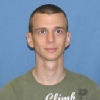
\includegraphics[width=0.2\textwidth]{joel.jpg}
\end{centering}
\end{wrapfigure}
I'm a student in the PhD program in the Applied Mathematics and Statistics department here at Stony Brook University. I use programming every day in my research into numerical methods for relativistic quantum chemistry. I took my first programming course (in Python!) my senior year in high school, and now I primarily program in C++.

\subsection*{Marisa Lim} 
\begin{wrapfigure}[6]{R}{0.2\textwidth}
%\begin{centering}
%    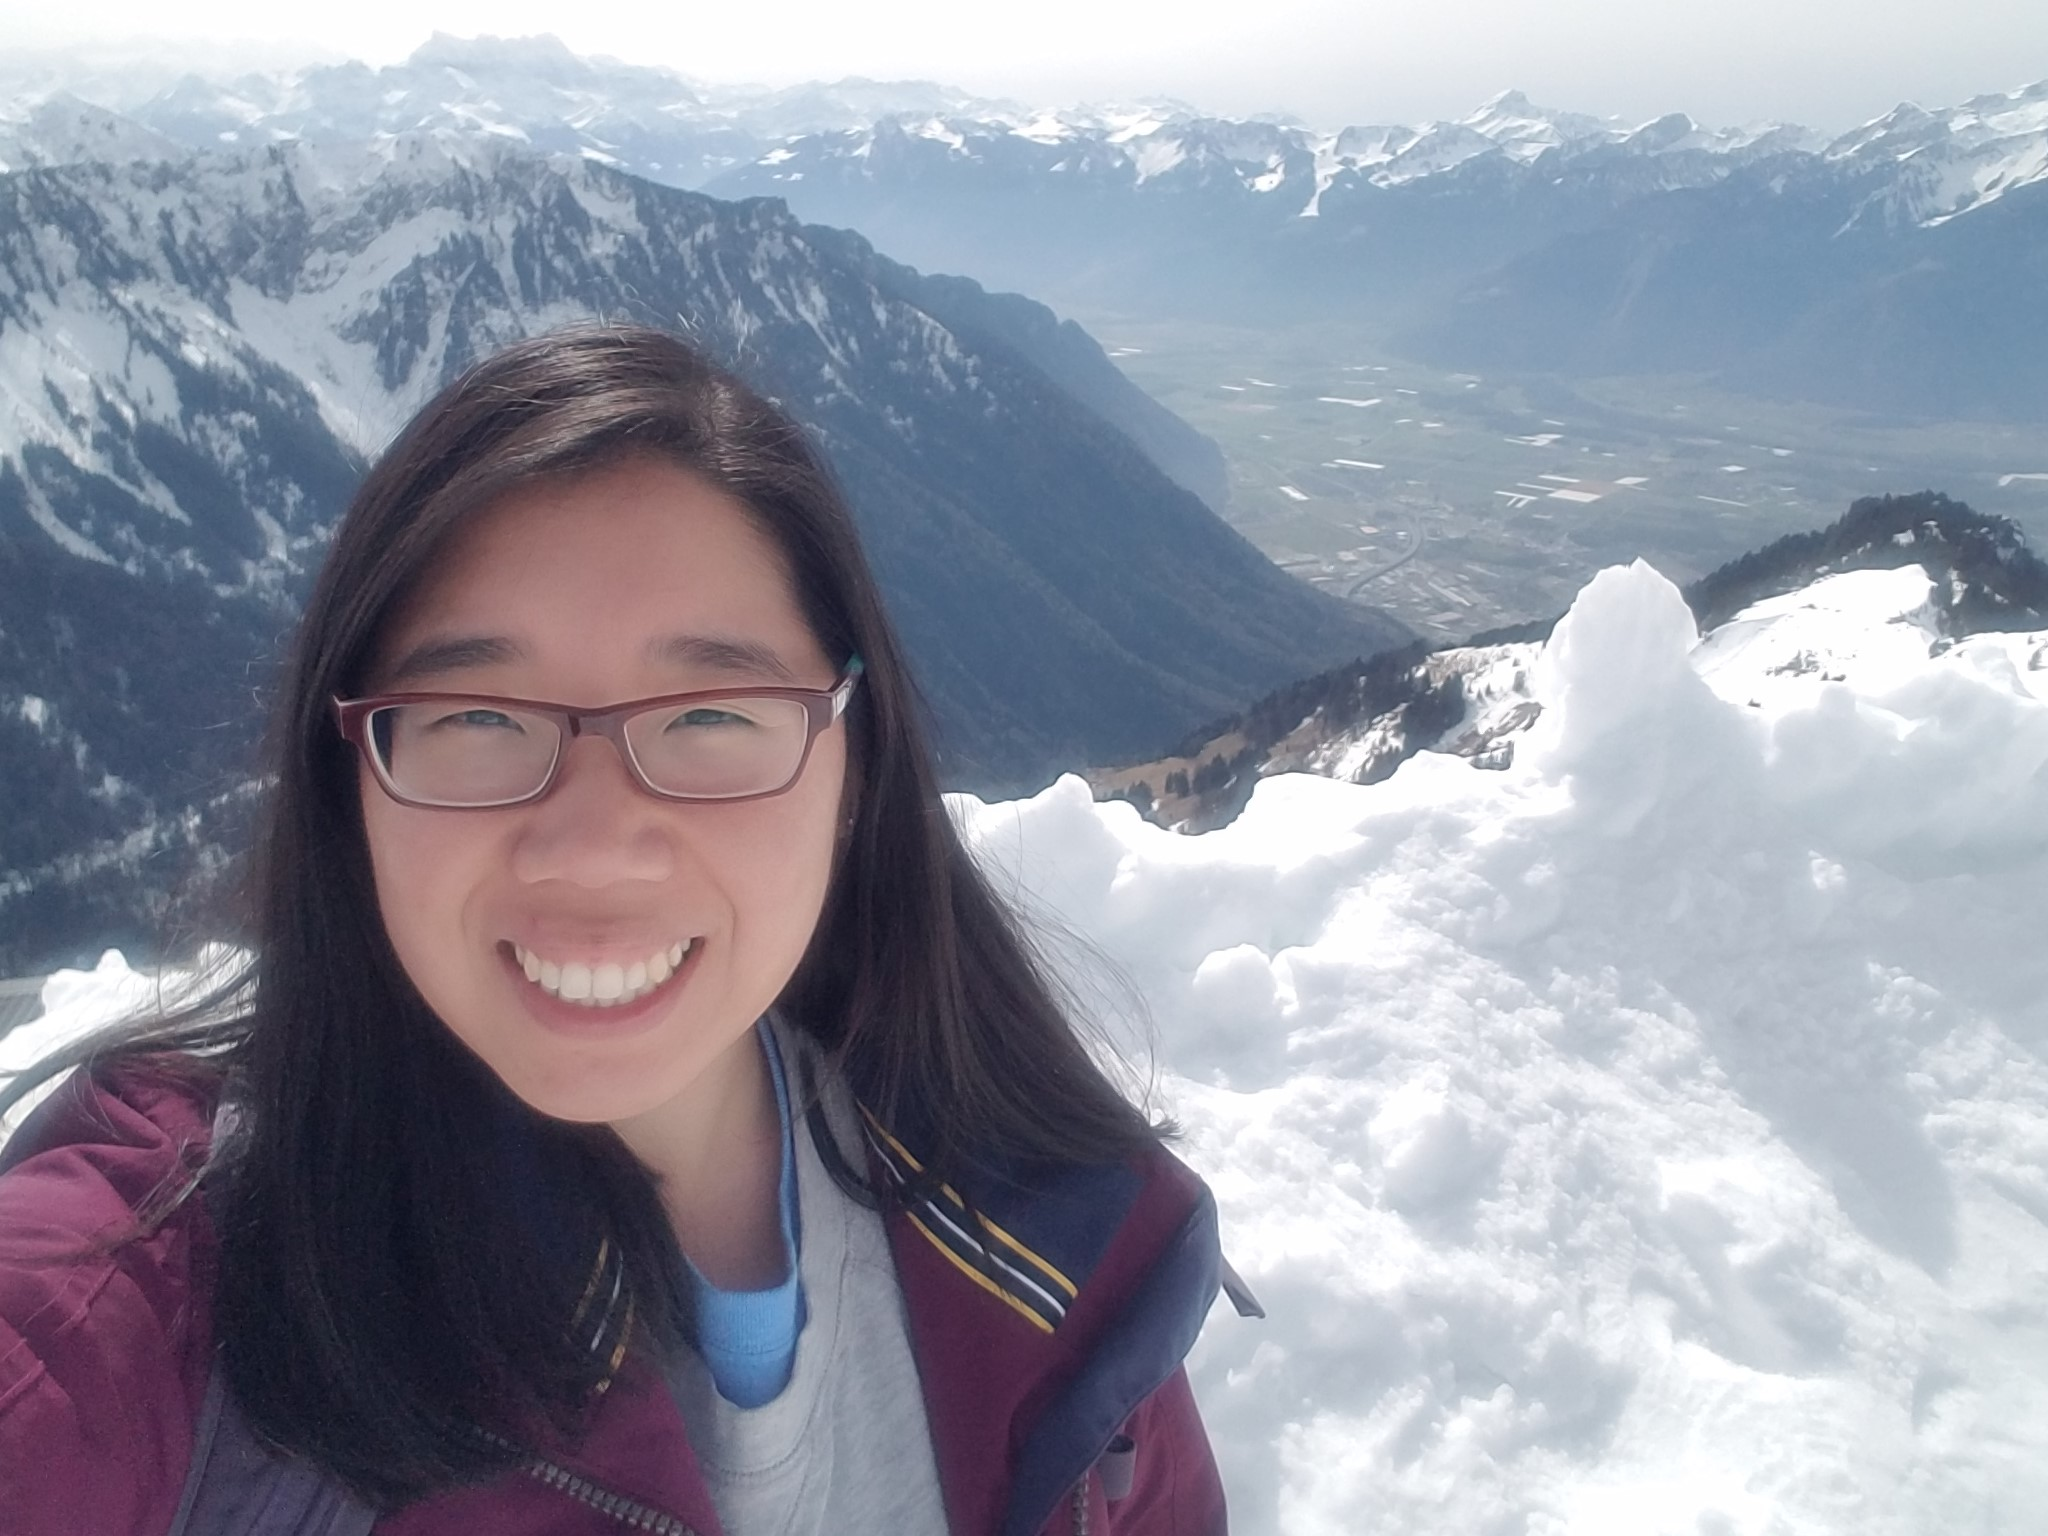
\includegraphics[width=0.2\textwidth]{marisa.jpg}
%\end{centering}
\end{wrapfigure}



\subsection*{Bryan Sundahl} 
\begin{wrapfigure}[4]{R}{0.2\textwidth}
\begin{centering}
    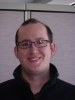
\includegraphics[width=0.2\textwidth]{bryan.jpg}
\end{centering}
\end{wrapfigure}
I'm a graduate student in Applied Math and Statistics here at Stony Brook University, working in the lab of Robert Harrison. My research involves creating software to model the response of molecules to external perturbations (\textit{e.g.} lasers).  Python is the main tool in my analysis of these models. 

\vspace{0.5 in}

\subsection*{Rebecca Uliasz} 
\begin{wrapfigure}{R}{0.2\textwidth}
\begin{centering}
    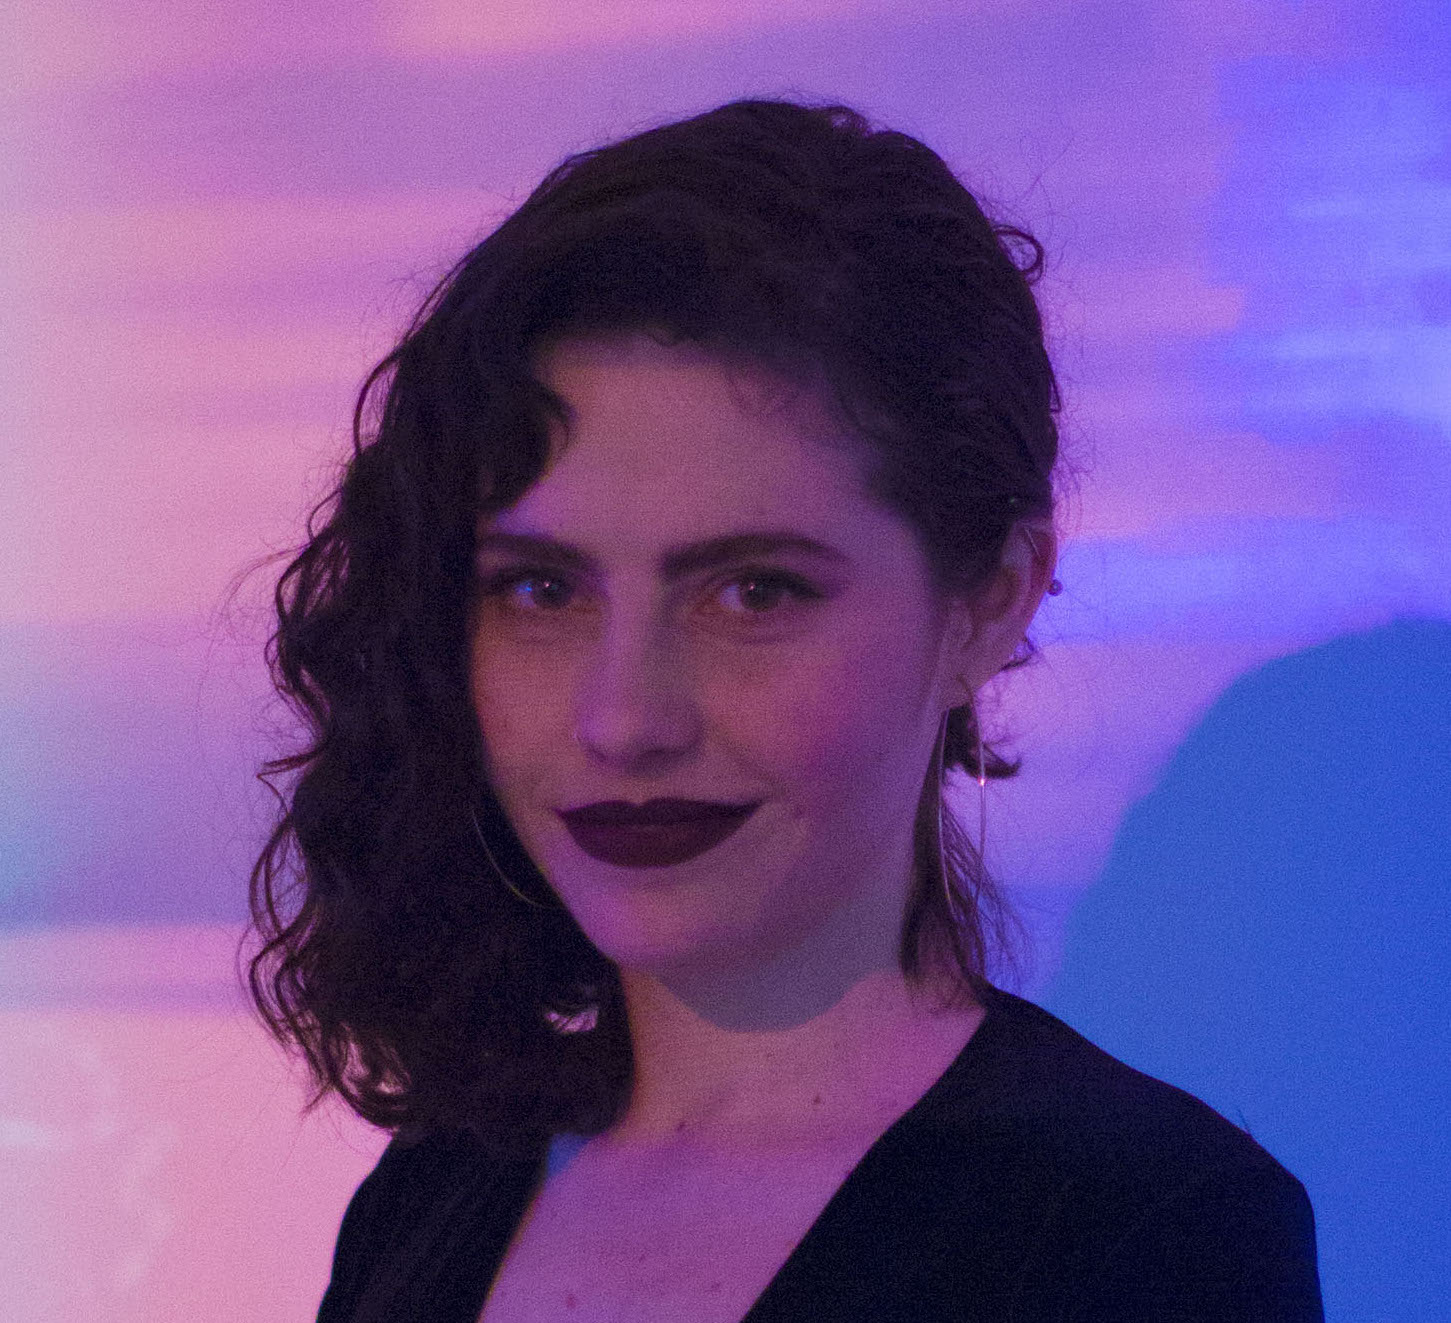
\includegraphics[width=0.2\textwidth]{rebecca.jpg}
\end{centering}
\end{wrapfigure}
I received an MFA in Studio Art at Stony Brook University this past spring. I create work involving multi-media installation, live stream, and digital modeling and animation. I use programming often to create custom software or to program hardware to use in interactive artworks. I am interested in video and audio synthesis, performance, and interface design and work mostly with visual programming languages like Max/MSP. 

\end{document}
